\documentclass[10pt, landscape]{article}
\usepackage[scaled=0.92]{helvet}
\usepackage{multicol}
\usepackage{calc}
\usepackage{ifthen}
\usepackage[landscape]{geometry}
%\usepackage{hyperref}

\usepackage{newtxtext} 

%for strikeout
\usepackage{ulem}

%For editing parbox
\usepackage[table]{xcolor}
%For editing itemise margins, reduce iterm separaion and list separation
\usepackage{enumitem}
% For math
\usepackage{amsmath,amsthm,amsfonts,amssymb}

%For pictures / figures
\usepackage{color,graphicx,overpic}
\graphicspath{ {./images/} }

%\usepackage{newtxtext} 
%\usepackage{amssymb}
%\usepackage[table]{xcolor}
%\usepackage{vwcol}
%\usepackage{tikz}
%\usepackage{wrapfig}
%\usepackage{makecell}

\pdfinfo{
  /Title (CS2107-notes.pdf)
  /Creator (Ger Teck)
  /Author (Ger Teck)
  /Subject ()
  /Keywords (tex)}

%% Margins for PAPER

% This sets page margins to .5 inch if using letter paper, and to 1cm
% if using A4 paper. (This probably isn't strictly necessary.)
% If using another size paper, use default 1cm margins.
\ifthenelse{\lengthtest { \paperwidth = 11in}}
	{ \geometry{top=.3in,left=.3in,right=.3in,bottom=.3in} }
	{\ifthenelse{ \lengthtest{ \paperwidth = 297mm}}
		{\geometry{top=0.5cm,left=0.5cm,right=0.5cm,bottom=0.5cm} }
		{\geometry{top=0.5cm,left=0.5cm,right=0.5cm,bottom=0.5cm} }
	}

% Turn off header and footer
\pagestyle{empty}
% for tight centres (less spacing)
\newenvironment{tightcenter}{%
  \setlength\topsep{0.5pt}
  \setlength\parskip{0.5pt}
  \begin{center}
}{%
  \end{center}
}

% Redefine section commands to use less space
\makeatletter
\renewcommand{\section}{\@startsection{section}{1}{0mm}%
                                {-1ex plus -.5ex minus -.2ex}%
                                {0.5ex plus .2ex}%x
                                {\normalfont\large\bfseries}}
\renewcommand{\subsection}{\@startsection{subsection}{2}{0mm}%
                                {-1explus -.5ex minus -.2ex}%
                                {0.5ex plus .2ex}%
                                {\normalfont\normalsize\bfseries}}
\renewcommand{\subsubsection}{\@startsection{subsubsection}{3}{0mm}%
                                {-1ex plus -.5ex minus -.2ex}%
                                {1ex plus .2ex}%
                                {\normalfont\small\bfseries}}
% change font
%\renewcommand{\familydefault}{\sfdefault}
%\renewcommand\rmdefault{\sfdefault}
\linespread{1.05}

\makeatother

% Define BibTeX command
\def\BibTeX{{\rm B\kern-.05em{\sc i\kern-.025em b}\kern-.08em
    T\kern-.1667em\lower.7ex\hbox{E}\kern-.125emX}}

% Don't print section numbers
\setcounter{secnumdepth}{0}

\setlength{\parindent}{0pt}
\setlength{\parskip}{0pt plus 0.5ex}

%% this changes all items (enumerate and itemize, reduce margins) ITEMIZE SEPARATION HERE
\setlength{\leftmargini}{0.5cm}
\setlength{\leftmarginii}{0.5cm}
\setlist[itemize,1]{leftmargin=2mm,labelindent=1mm,labelsep=1mm, itemsep = 0mm}
\setlist[itemize,2]{leftmargin=4mm,labelindent=1mm,labelsep=1mm, itemsep = 0mm}

%itemsep = 0mm
%\setlist{nosep}

% -------------------------------------------------------------------------------

% START OF DOCUMENT HERE

\begin{document}
\raggedright
\footnotesize
\begin{multicols*}{3}

% multicol parameters
% These lengths are set only within the two main columns
%\setlength{\columnseprule}{0.25pt}
\setlength{\premulticols}{1pt}
\setlength{\postmulticols}{1pt}
\setlength{\multicolsep}{1pt}
\setlength{\columnsep}{2pt}


%% DOCUMENT NAME HERE
\begin{center}
     \Large{\textbf{CS2107 Introduction to \\
     				 Information Security}} \\
\end{center}
AY24/25 Sem 2, github.com/keithxun


\section{Alice Opens Browser and Visits URL}

\subsection{Phishing Attack: Social Engineering}
Trick the user to visit a website which is a spoofed canvas login page
\begin{itemize}
\item Typo squatting: Attacker register domain names that are similar to legitimate domain names but with typo error.
\item Subdomain Takeover: Users may be tricked into visiting these look-alike subdomains (*.attacker.com) instead of (*.com)
\end{itemize}

\subsection{Phishing Attack: SSL Bug}
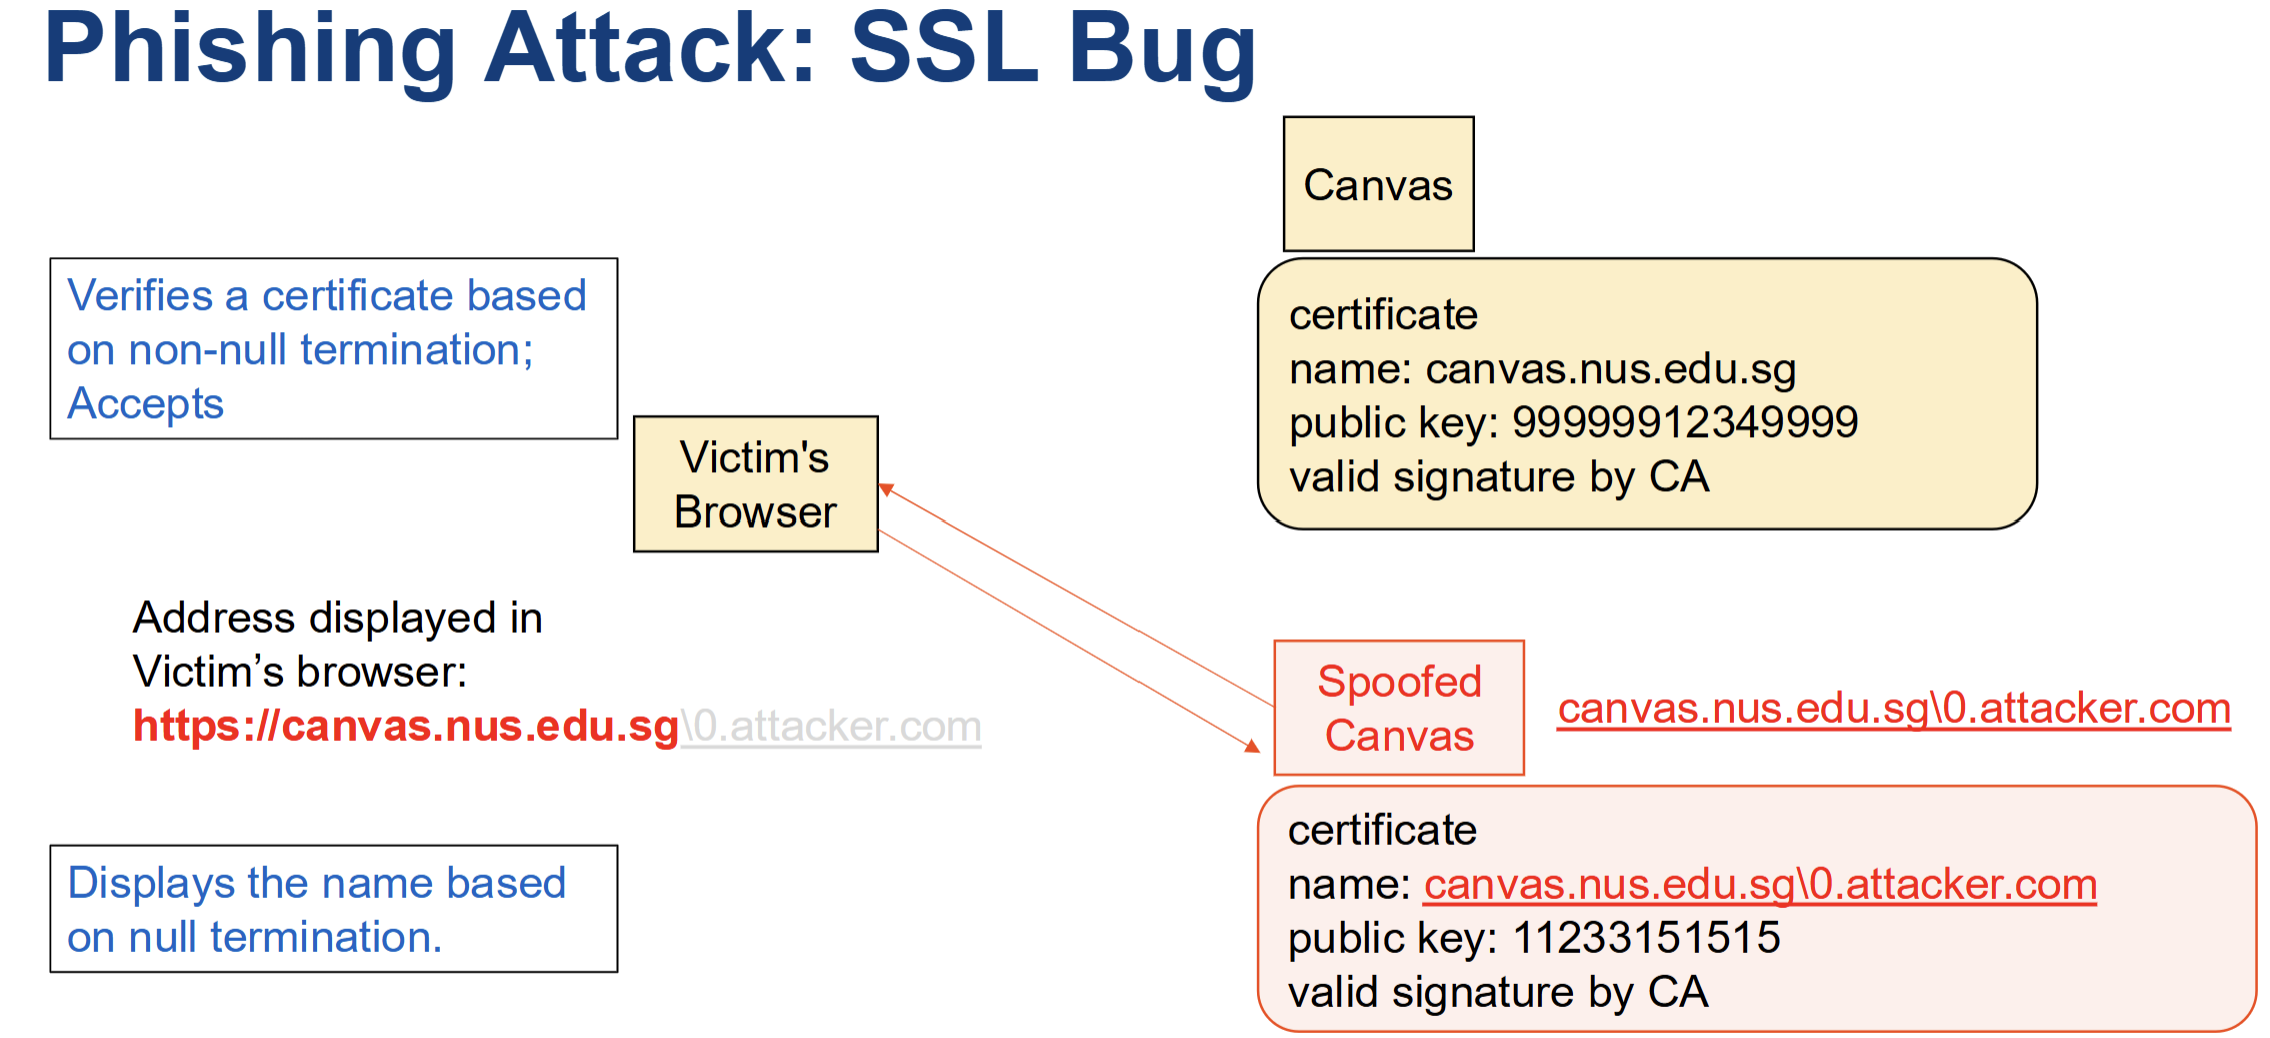
\includegraphics[width=\columnwidth]{SSL Bug.png}

\subsection{Countermeasures}
\begin{itemize}
	\item User training: Workshops, reminders
	\item Blacklisting: Repositary site keeping lists of phising sites
\end{itemize}

\section{Attacker in the Same Local Network}

\subsection{DNS Spoofing}
DNS has no confidentiality, integrity, or authentication.
\begin{itemize}
	\item Manipulate DNS response to redirect users to a fake website
	\item Same cafe (Physical layer), On-path router (IP layer)
	\item Capability: Attacker able to send fake response before the actual one
\end{itemize}

\subsection{Countermeasures}
\begin{itemize}
	\item DNSSEC: Digital signature for DNS records for authenticity and integrity
	\item DoH: DNS over HTTPS for confidentiality
	\item DoT: DNS over TLS
	\item DoQ: DNS over QUIC
\end{itemize}

\subsection{ARP Spoofing}
ARP requests are broadcasted to all hosts in the same local network. Attacker can send fake ARP responses to trick the victim
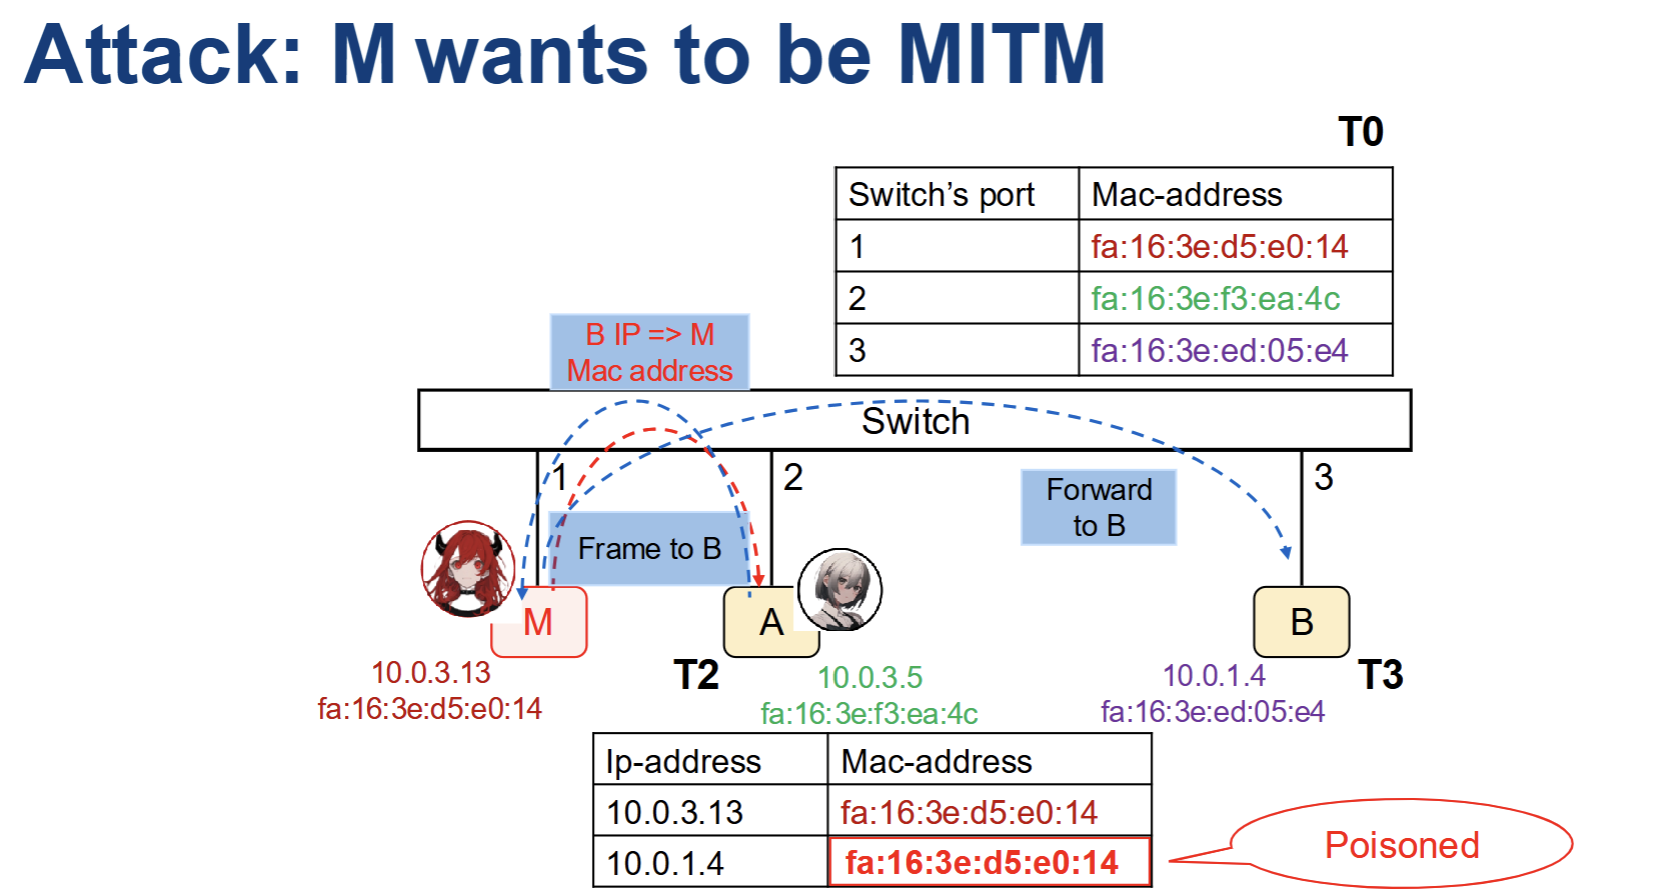
\includegraphics[width=\columnwidth]{ARP Poisoning.png}
\begin{itemize}
	\item Attacker poisons the ARP tables so as to gain MITM access
	\item Attack is present in the local network (Physical Layer) and able to send ARP responses
\end{itemize}

\subsection{Countermeasures}
\begin{itemize}
	\item Static ARP entries: Manually configure the ARP table
	\item Packet filtering: Only allow ARP requests from trusted hosts, block single MAC address associated to multiple IPs
\end{itemize}	

\subsection{DDOS: Smurf Attack}
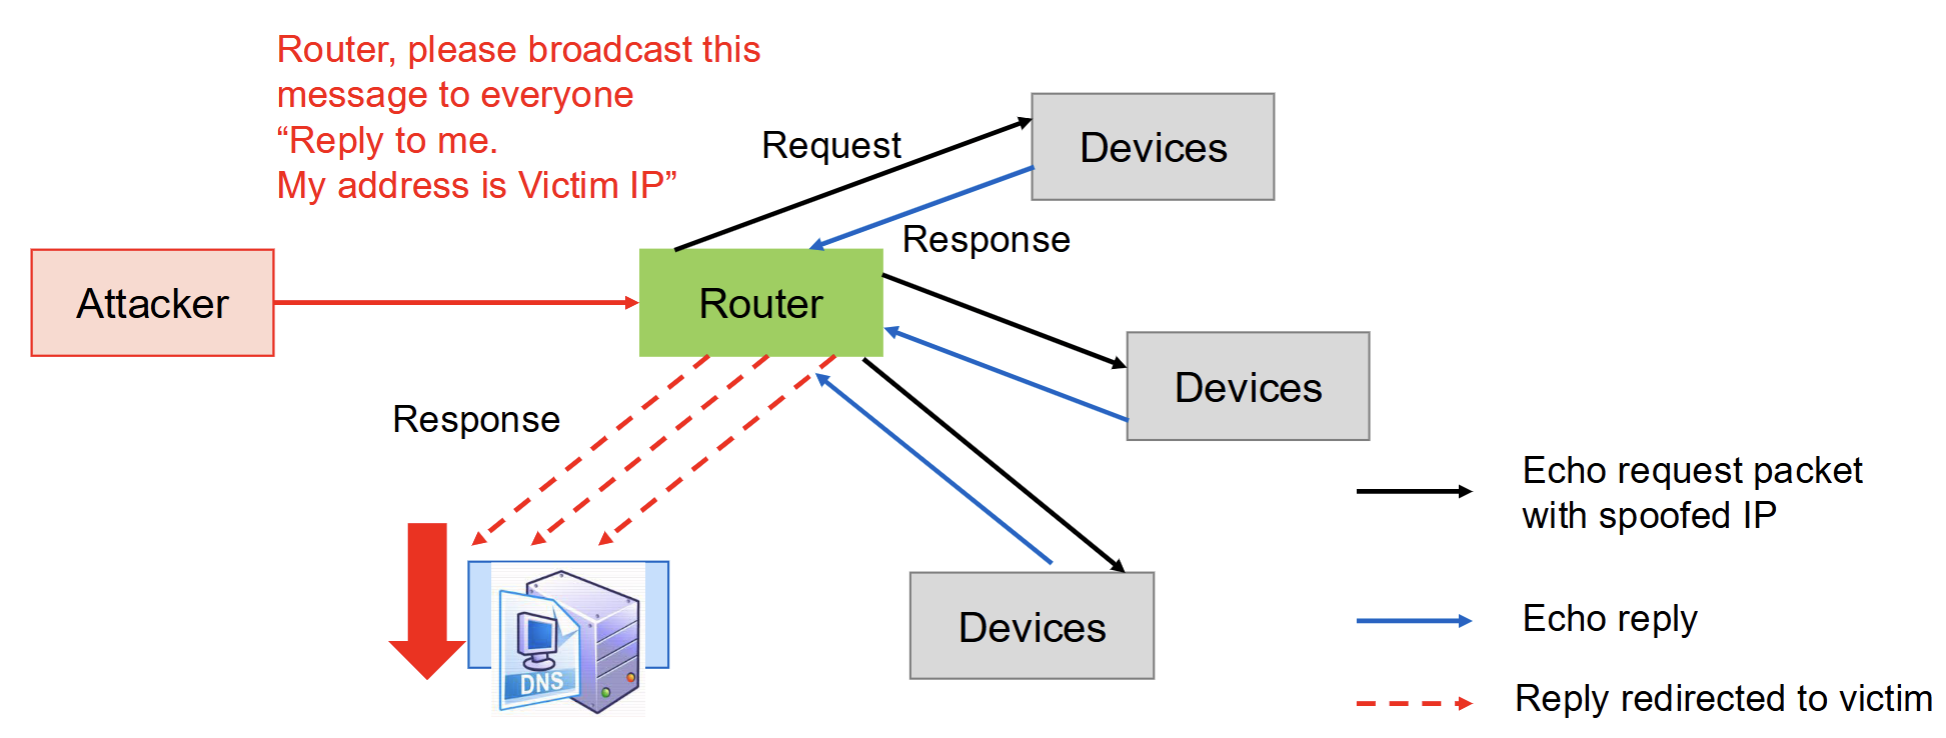
\includegraphics[width=\columnwidth]{Smurf Attack.png}

\subsection{DDOS: Amplification Attack}
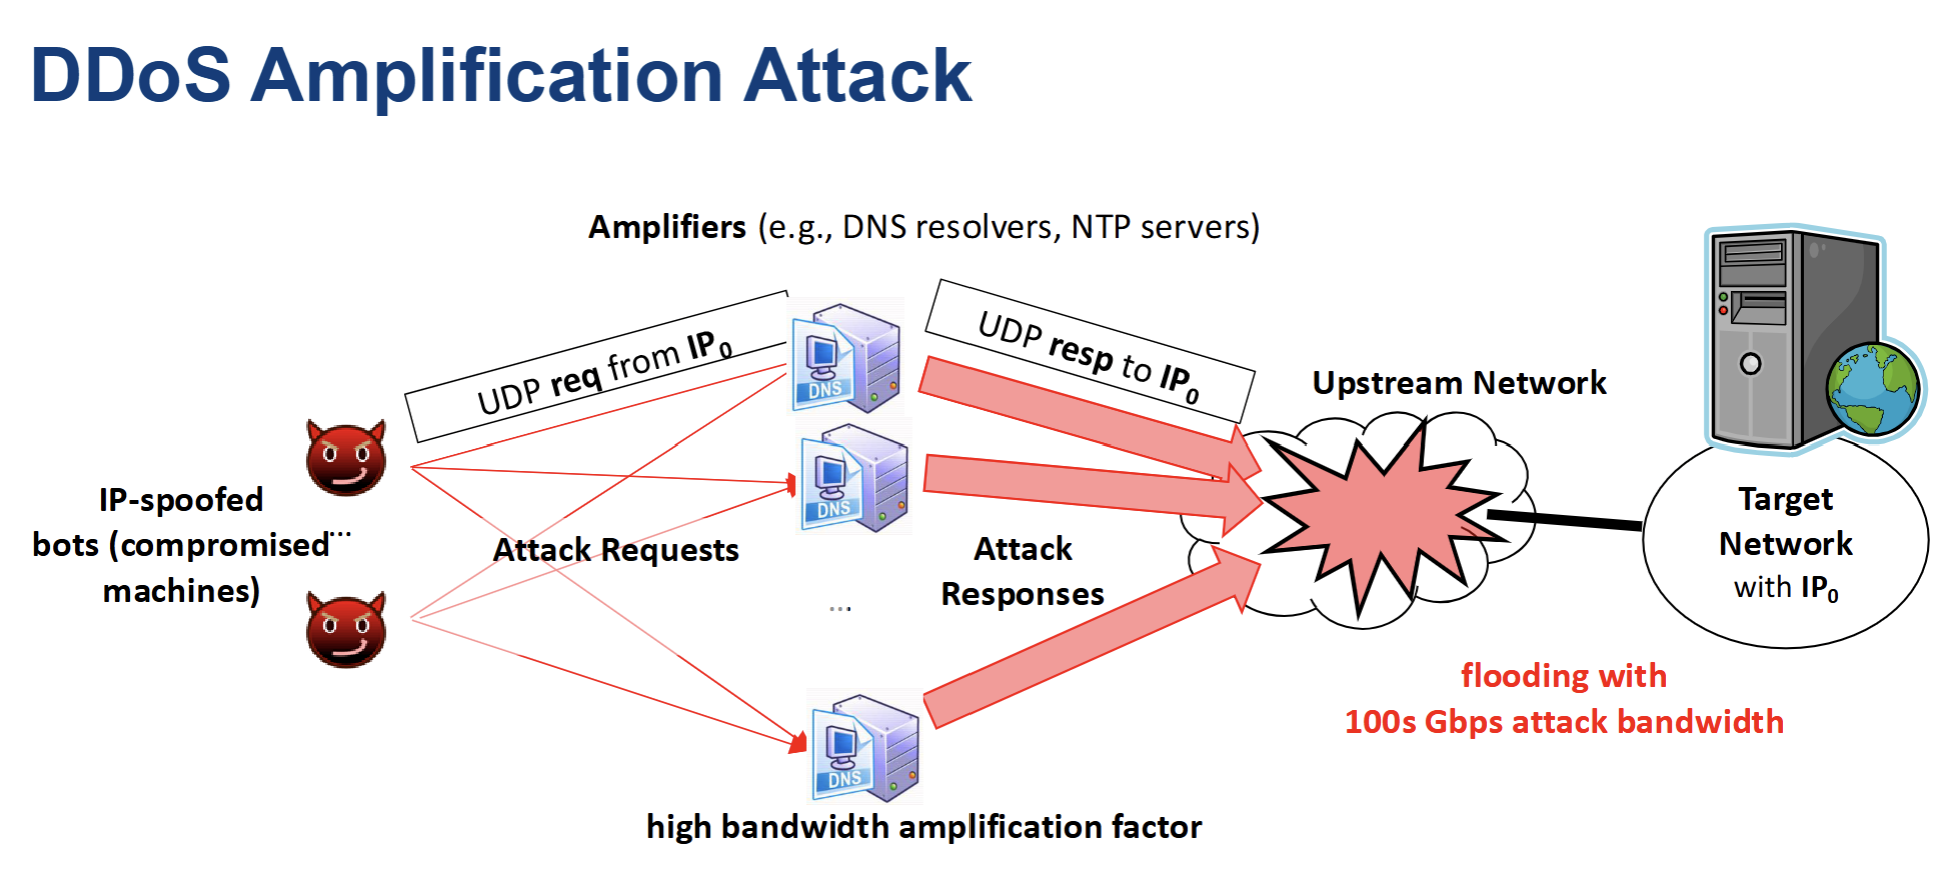
\includegraphics[width=\columnwidth]{Amplification Attack.png}

\subsection{Countermeasures}
\begin{itemize}
	\item configure firewalls to block incoming ICMP Echo requests packets directed at broadcast addresses
	\item Redundant servers, rate limiting, etc
	\item Load balancing for amplification attack
\end{itemize}

\section{Establishing HTTP Session}

\subsection{Certificates}
\begin{itemize}
	\item Certificate binds an entity to some public key (Identity, public key, validity period)
	\item Certificate Authority (CA) is a trusted third party that issues digital certificates
	\item CA signs the certificate with its private key
	\item CA's public key is distributed to all users
	\item Self-signed certificate: CA is the entity itself
	\item Domain Validated certificate: Least stringent validation, only verifies if applicant owns the domain
	\item Extended Validation certificate: More stringent validation, Includes organization details, registration number and jurisdiction etc
\end{itemize}

\subsubsection{MITM due to Rogue CA}
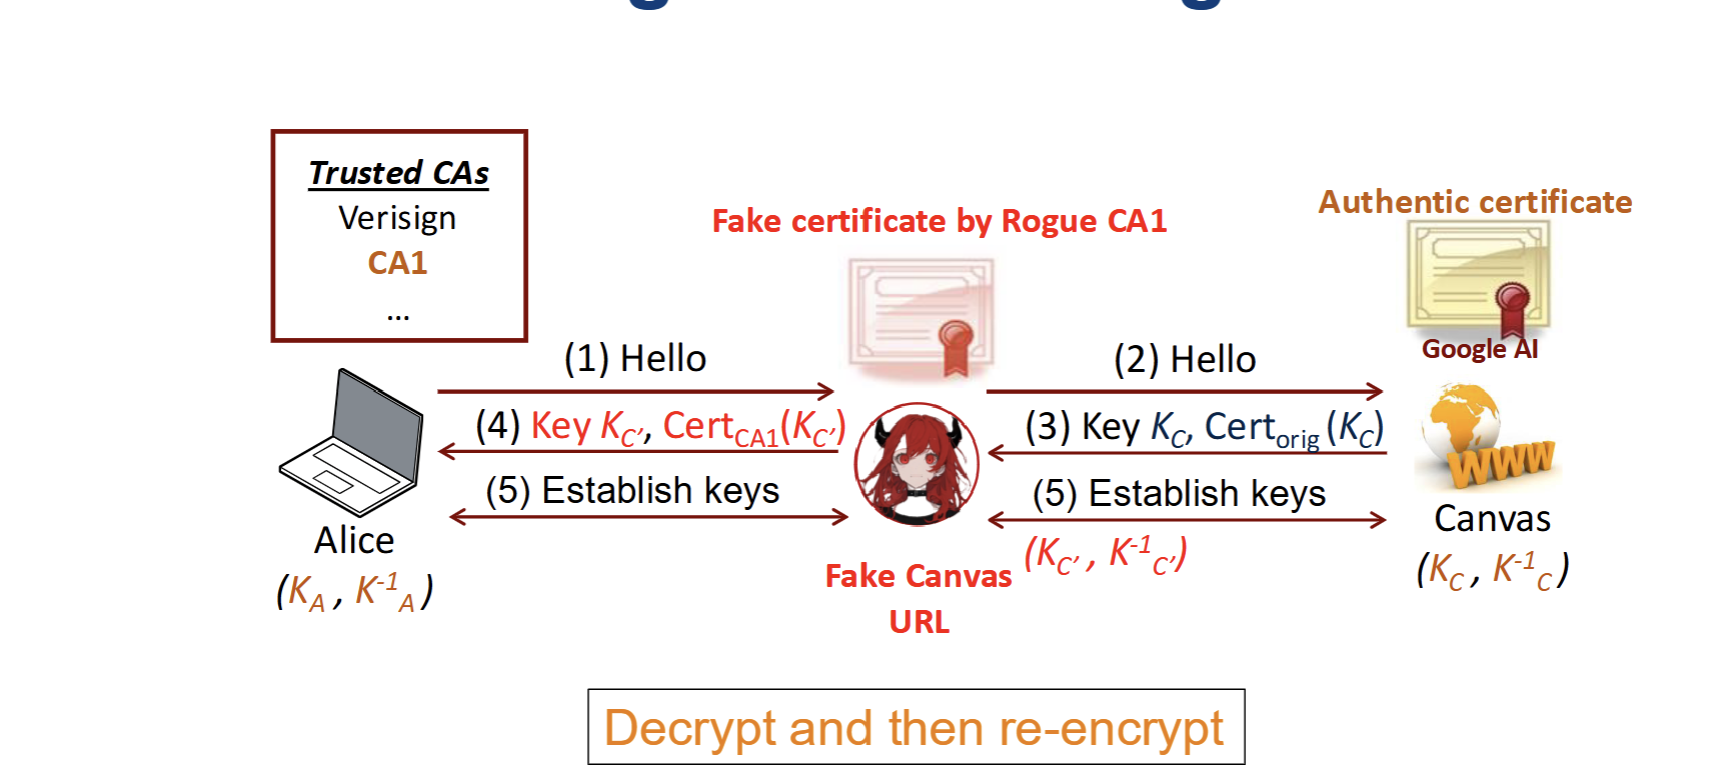
\includegraphics[width=\columnwidth]{Rogue CA.png}

\subsection{Countermeasures}
\begin{itemize}
	\item Certificate Revocation: To invalidate certificates (OCSP, CRL)
	\item Short-lived certificate: No need to revoke
	\item Certificate Log: Public, verifiable, and append-only log of certificates
\end{itemize}

\section{Security Principle}
confidentiality, integrity, availability
\begin{itemize}
	\item Confidentiality: Only authorized parties can access the data
	\item Integrity: Data is not modified by unauthorized parties
	\item Availability: Authorized parties can access the data when needed
\end{itemize}

\subsection{Confidentiality}
\begin{itemize}
	\item Symmetric Encryption scheme: Same key for encryption and decryption
	\item Substitution and Permutation: Not secure - Brute force, CTO, KPA
	\item One-time Pad: Theoretical, secure under certain conditions
	\item Stream cipher: Not secure if key is reused, needs IV 
	\item DES (not secure), AES (secure)
	\item MITM on DES: Ecrypt from one side, decrypt from the other side
	\item Padding Oracle Attack: Mask = New pad xor old pad, actual = new pad xor mask 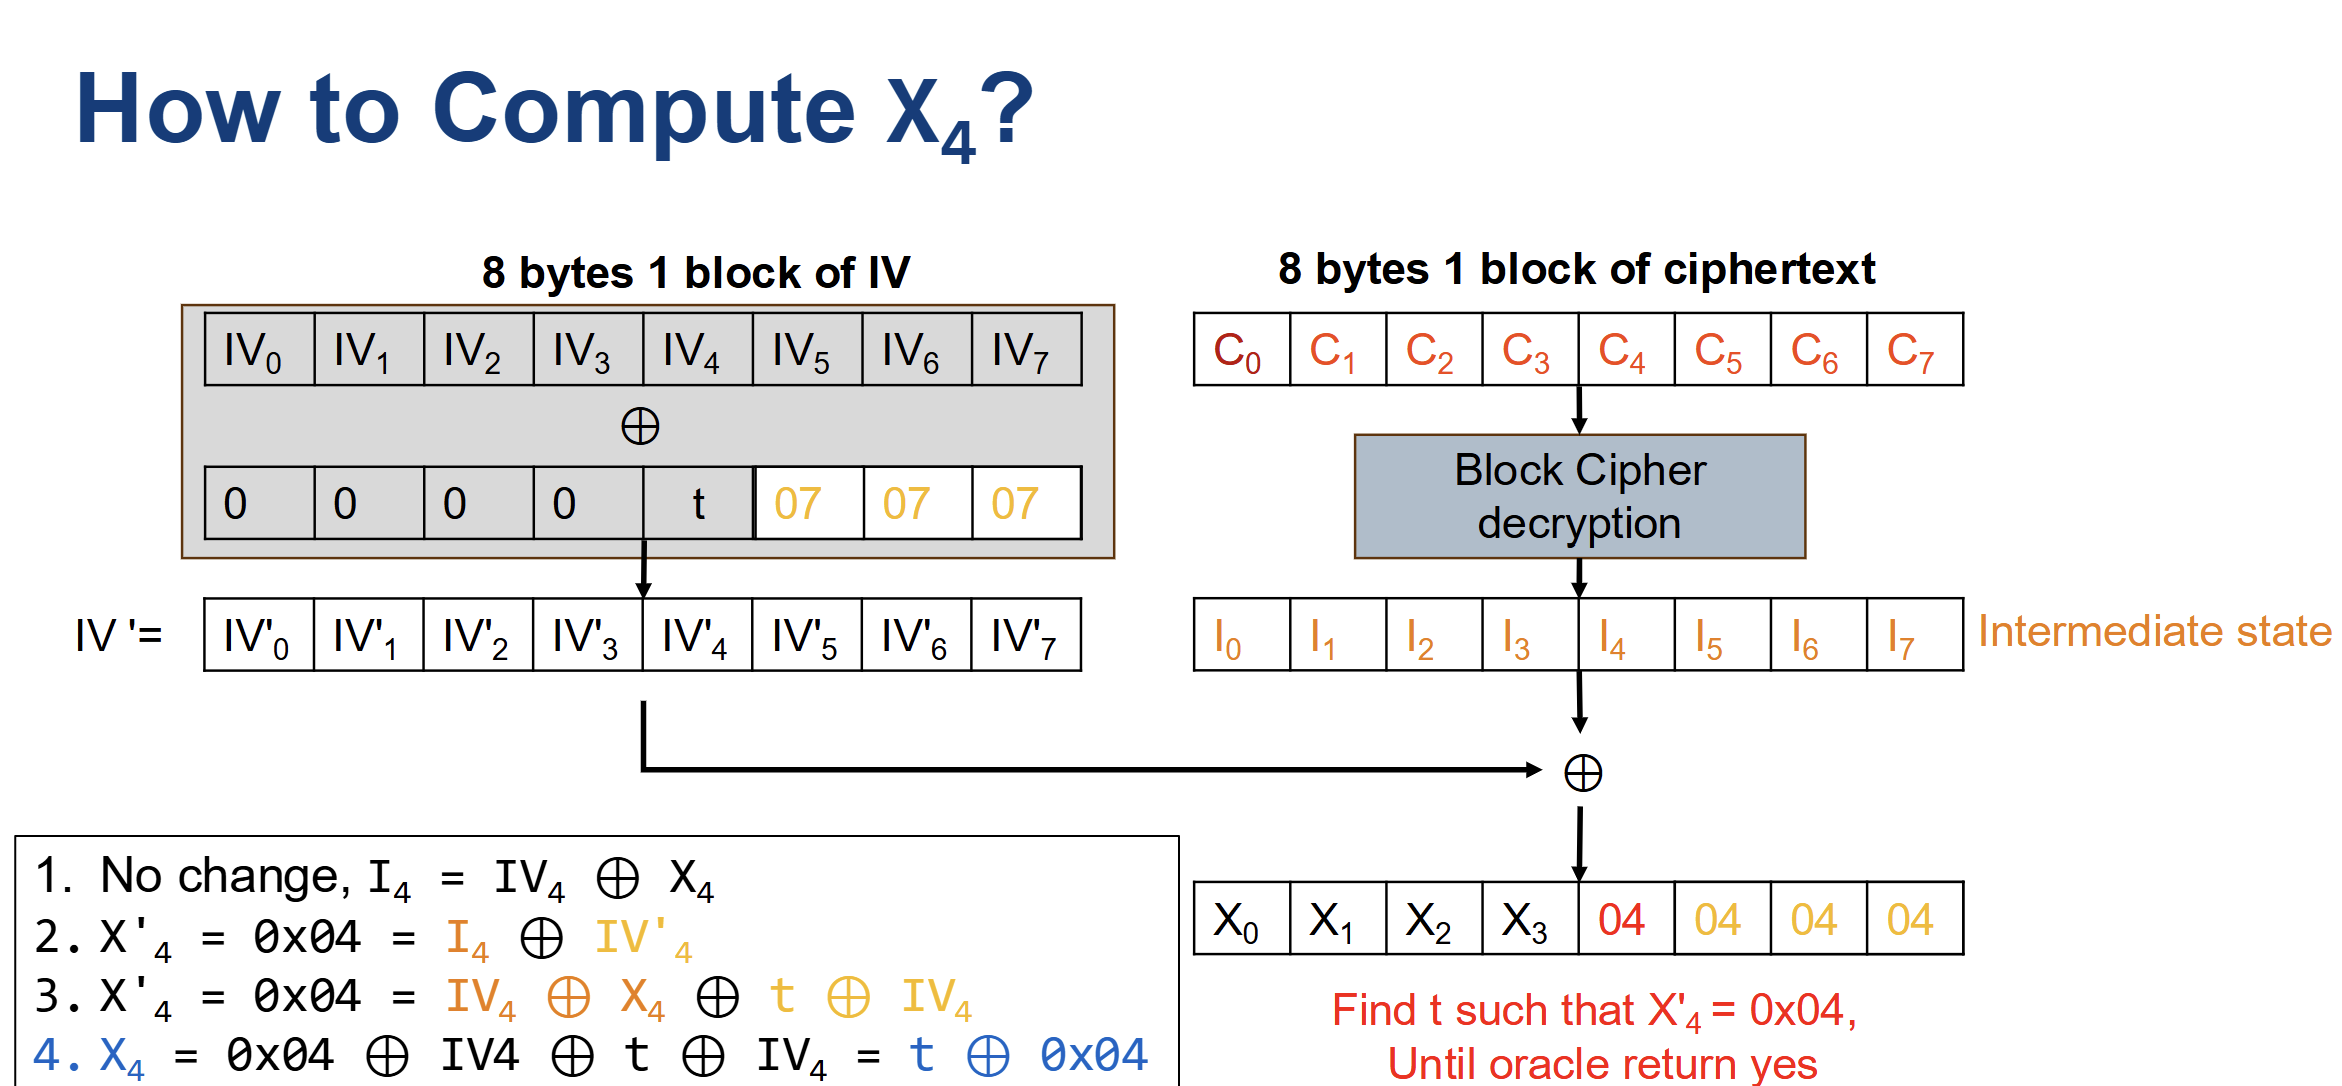
\includegraphics[width=\columnwidth]{Padding Oracle.png}
	\item Asymetric Encryption scheme: Different keys for encryption and decryption
	\item RSA: Integer factorization problem, multiplying two large primes to generate n is easy but factoring n is hard
	\item $n = pq$, $\phi = (p-1)(q-1)$, $e$ = public exponent, $d$ = private exponent such that $\gcd(e, \phi) = 1$ and $ed \bmod \phi = 1$
	\item $c = m^e \bmod n$, $m = c^d \bmod n$
	\item RSA is significantly slower than AES
	\item Bell-LaPadula Model: No read up, no write down
\end{itemize}

\subsection{Integrity}
\begin{itemize}
	\item Hash: No authentication
	\item MAC: Authentication and integrity, keyed, symmetric 
	\item Signature: Authentication and integrity, asymmetric, non-repudiation
	\item Birthday attack: Find collision after $1.17 \times 2^{n/2}$ hashes
	\item Collision resistance: No 2 inputs produce the same hash
	\item Pre-image resistance: Cannot get the input from the hash
	\item Second pre-image resistance: Given an input, cannot find another input that produces the same hash
	\item Biba Model: No write up, no read down
\end{itemize}

\subsection{Authenticated Key Exchange}
\begin{itemize}
	\item Station to Station Protocol: Deffie Hellman key exchange protocol, not secure against MITM, forward secrecy 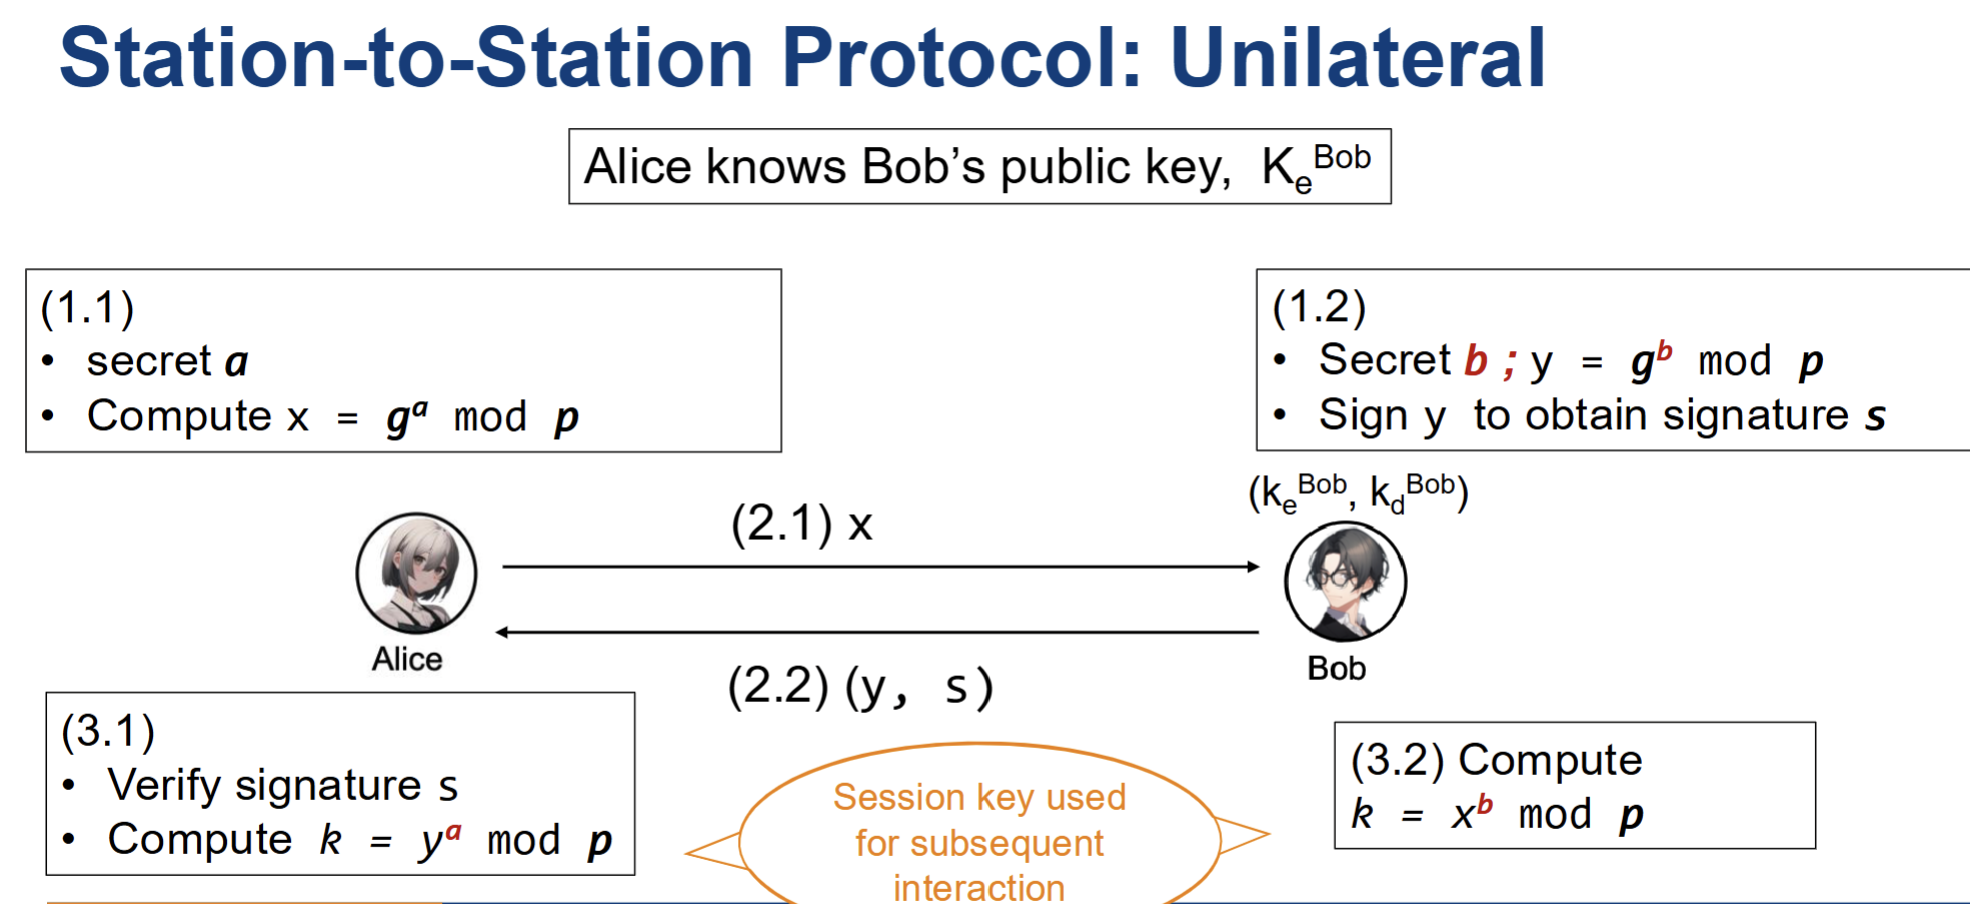
\includegraphics[width=\columnwidth]{STS.png}
	\item MITM attack: Attacker intercepts the public keys and sends his own public key to both parties
	\item PKC-based Key Exchange: No forward secrecy 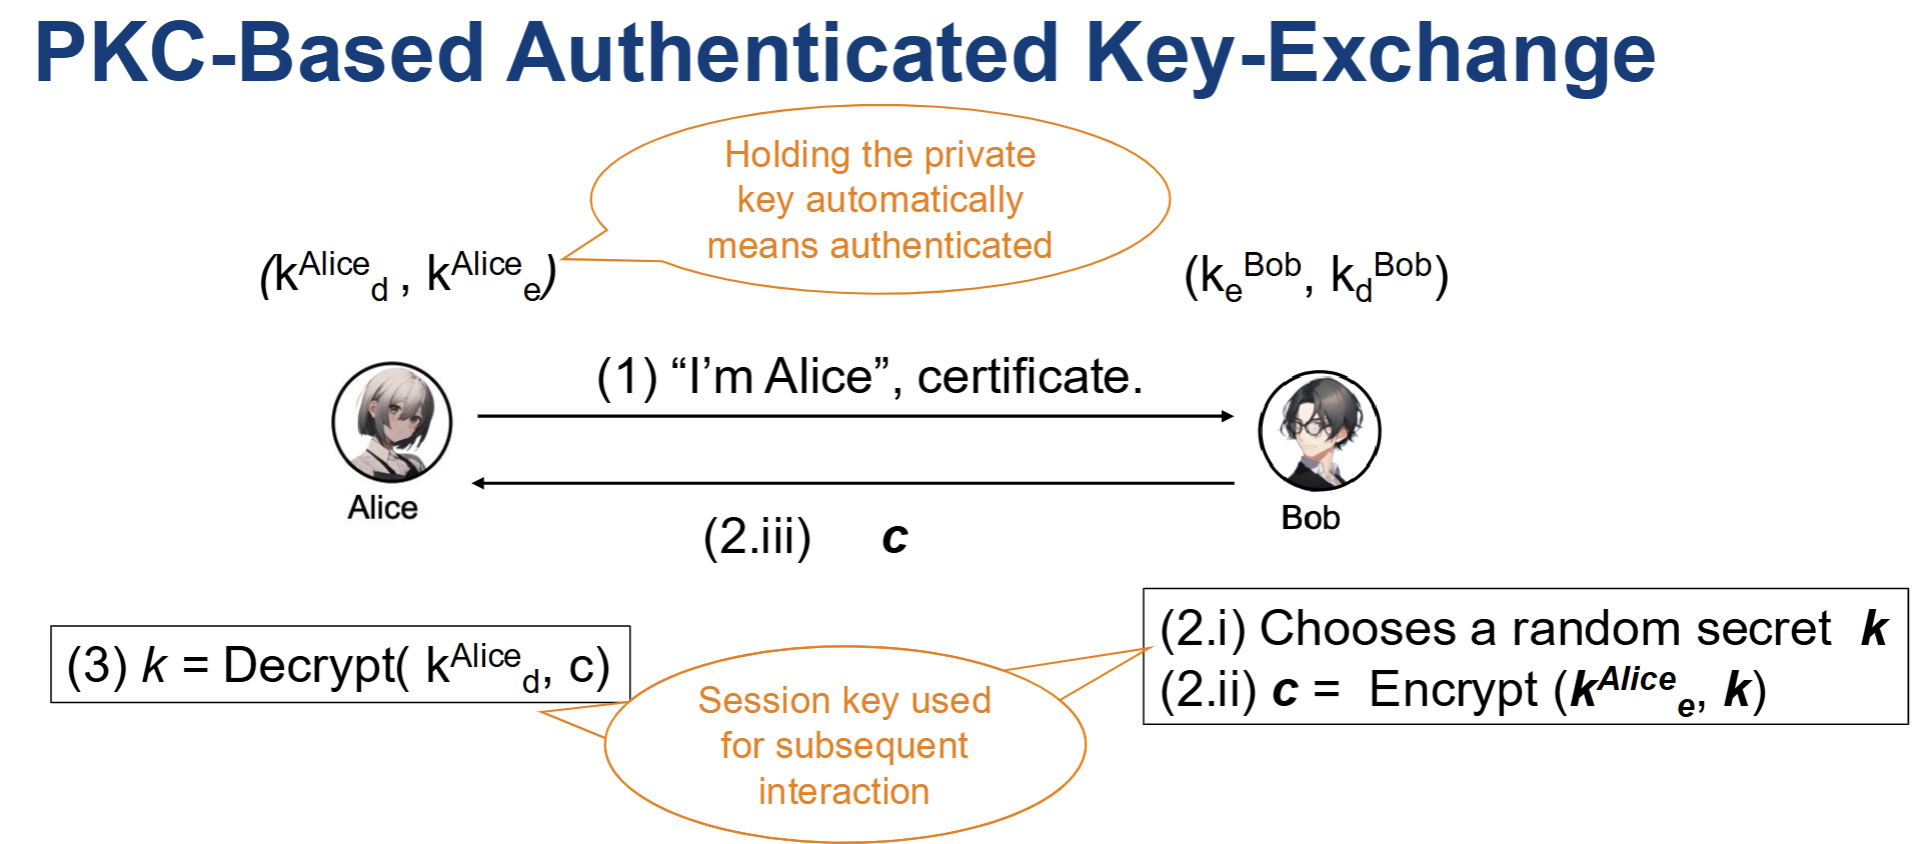
\includegraphics[width=\columnwidth]{PKC key exchange.png}
	\item Perfect forward secrecy: Even if the private key is compromised, past sessions are still secure 
\end{itemize}

\subsection{Authenticated Encryption}
\begin{itemize}
	\item Encrypt-then-MAC: Encrypt the message first, then MAC it, secure and can verify MAC before decrypting
	\item MAC-then-encrypt: MAC the message first, then encrypt it, not secure, no ciphertext integrity
	\item Encrypt-and-MAC: Encrypt and MAC at the same time, not secure, no ciphertext integrity
	\item SSL/TLS protects data in transport layer
	\item IPsec protects data in network layer
	\item WPA2 protects data over Wi-Fi between link and physical layer
	\item VPN tunnel at layer 3 (IP layer) to further improve security, hides everything but src mac and dest mac
\end{itemize}

\section{Passwords}
\begin{itemize}
	\item Bootstrapping: Establishing common password 
	\item Entropy: $H = \text{Password Length} \times \log_2(\text{Symbol Set Size})$
	\item 2FA: Something you know, something you have, something you are. Different from multi-step verification
	\item Attack on Password reset: If reset link is constructed by taking the domain name from the host header of http request without validation, attacler post request to host and gets victim's otp
	\item Online attack (rate limit) vs Offline attack (Add salt and hash)
\end{itemize}

\section{Cookies}
Choice of token should include mac computed using server secret key 
Same origin matches protocol, hostname and port number. Same site matches protocol and last part of hostname only (String comparison www. matters)

\subsection{Properties}
\begin{itemize}
	\item Domain: Domain that can access the cookie
	\item Path: Path that can access the cookie
	\item Secure: Only sent over encrypted HTTPS
	\item HttpOnly: Not accessible via JavaScript
	\item SameSite (Strict or lax): Prevent CSRF attacks
	\item Expiration date: When the cookie expires
\end {itemize}

\subsection{CSRF}
\begin{itemize}
	\item Victim has logged into the site and has a valid session cookie
	\item Victim clicks a malicious link to attacker's site
	\item Malicious site issue a stealthy request to the target site
\end{itemize}

\subsection{Countermeasures}
\begin{itemize}
	\item SameSite cookie: Prevents CSRF attacks by not sending cookies with cross-site requests
	\item CSRF token: Unique token for each request, sent as a hidden field in the form
	\item Referer header: Check if the request is coming from the same site
\end{itemize}

\subsection{XSS}
\begin{itemize}
	\item Reflected XSS: Attacker injects malicious script into the URL, victim clicks the link and the script is executed
	\item Stored XSS: Attacker injects malicious script into the website, victim visits the website and the script is executed
	\item Attacker tricks user to click on malicious link, which contains the target website and a malicious script
	\item Server constructs a response html that contains the script and browser then runs the script
\end{itemize}

\subsection{Countermeasures}
\begin{itemize}
	\item Input validation: Validate all user inputs
	\item HttpOnly cookie: Prevents JavaScript from accessing the cookie
\end{itemize}

\subsection{SQL Injection}
\begin{itemize}
	\item Attacker injects malicious SQL code into the input field
	\item Server constructs a SQL query that contains the malicious code
	\item Attacker can manipulate the database
	\item Example: Attacker enters "bob' OR 1=1; --" in the input field
	\item Server constructs a SQL query that looks like this: "SELECT * FROM User WHERE name = ' " + userinput1 + " ' AND password = ' " + userinput2 + " '";
	\item The query returns all users in the database
\end{itemize}

\subsection{Countermeasures}
Parameterized queries: Use prepared statements to prevent SQL injection

\section{Access Control}

\subsection{Exploit software vulnerabilities}
\begin{itemize}
	\item Stack overflow: Attacker injects malicious code into the stack (Carnaries, memory randomization)
	\item Integer overflow: Leads to unintended behaviour
	\item Format string attack: Attacker injects malicious format string into the input field
	\item Unsafe functions such as gets, scanf, sprintf
\end{itemize}

\subsection{Time of Check to Time of Use}
Attacker can exploit the time gap between checking the access control and using the resource by deleting the original file and creating a link with the same name

\subsection{Countermeasures}
\begin{itemize}
	\item Avoid separate system calls for checking and using the resource
	\item Set effective UID to the appropriate user
\end{itemize}


\end{multicols*}
\end{document}
